\documentclass[9pt,aspectratio=169,xcolor=table]{beamer}
\usepackage[compact]{styles/stmcommon}

\title{Synchronous Serial Interfaces: SPI and $I^2$C}
\subtitle{\emph{Introduction to ARM Cortex-M Microprocessors} --- Chapter 13}

\begin{document}

\titlepage

%===============================================================================
\section{Why This Matters}
%===============================================================================

\begin{frame}{Why This Chapter Matters}
    \begin{columns}[T]
    \begin{column}{.47\textwidth}
        {\normalsize UART has no clock wire, so both ends must agree on the baud rate. Adding a clock wire removes that need and the speed limit. SPI is fast and simple, but costs one pin per device. $I^2$C is slower, yet it connects dozens of devices on two wires. You will read a real sensor and turn its raw values into a physical measurement.}
    \end{column}
    \begin{column}{.51\textwidth}
        \begin{block}{After this chapter, you can:}
        {\small
        \begin{enumerate}\itemsep2pt
            \item Name the four SPI signals; explain full-duplex exchange.
            \item Choose CPOL and CPHA; calculate $f_{\text{SCK}}$.
            \item Configure an SPI master and do a register transaction.
            \item Describe the $I^2$C phases; explain open-drain and pull-ups.
            \item Configure an $I^2$C master and read a slave register.
            \item Choose between SPI and $I^2$C, and justify it.
            \item Convert a real sensor's output to engineering units.
        \end{enumerate}}
        \end{block}
    \end{column}
    \end{columns}
\end{frame}


%===============================================================================
\section{The SPI Bus}
%===============================================================================

\begin{frame}{Four Wires, Full Duplex}
    \begin{columns}[T]
    \begin{column}{.46\textwidth}
        \begin{center}
        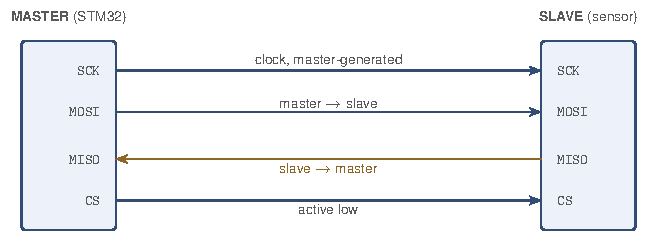
\includegraphics[width=\textwidth]{assets/spi-bus.pdf}
        \end{center}
    \end{column}
    \begin{column}{.5\textwidth}
        {\small
        \striped
        \begin{tabular}{@{}l l@{}}
            \toprule
            \textbf{Signal} & \textbf{Direction} \\
            \midrule
            \texttt{SCK}  & Master $\rightarrow$ slave \\
            \texttt{MOSI} & Master $\rightarrow$ slave \\
            \texttt{MISO} & Slave $\rightarrow$ master \\
            \texttt{CS}   & Master $\rightarrow$ slave, \alert{per device} \\
            \bottomrule
        \end{tabular}}
    \end{column}
    \end{columns}

    \vspace{3mm}
    \begin{block}{A transfer is an \emph{exchange}, not a send}
        Master and slave are one \alert{circular shift register}. Every clock edge
        shifts a bit out of each and into the other --- so sending a byte
        \emph{always} receives one at the same time. To read a device you must
        still \alert{write something} (often a dummy byte) to generate the clock.
    \end{block}
\end{frame}

\begin{frame}[plain]{More Than One Slave}
    \begin{center}
    \includegraphics[width=.9\textwidth, height=.62\textheight, keepaspectratio]%
        {assets/spi-multi.pdf}
    \end{center}

    \vspace{1mm}
    {\small\centering \texttt{SCK}, \texttt{MOSI}, and \texttt{MISO} are
    \alert{shared} by every device; only chip select is \alert{private}.
    Adding a slave costs exactly one pin.\par}
\end{frame}

\begin{frame}[plain]{Full Duplex by Shift Register}
    \begin{center}
    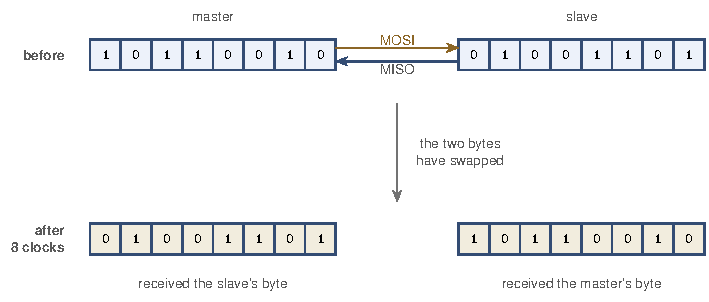
\includegraphics[width=.94\textwidth]{assets/spi-exchange.pdf}
    \end{center}

    \vspace{1mm}
    {\small\centering SPI is an \alert{exchange}, not a send or a receive. The
    two shift registers form one ring, so eight clock pulses trade their
    contents.\par}
\end{frame}


%===============================================================================
\section{Clock Polarity and Phase}
%===============================================================================

\begin{frame}[plain]{Clock Polarity and Phase}
    \begin{center}
    \includegraphics[width=.84\textwidth, height=.58\textheight, keepaspectratio]%
        {assets/spi-timing.pdf}
    \end{center}

    \vspace{2mm}
    {\small\centering \textbf{CPOL} sets the idle level of the clock;
    \textbf{CPHA} sets which edge samples the data. Four combinations, called
    \alert{modes 0 to 3} --- and the datasheet tells you which one your device
    needs.\par}
\end{frame}

\begin{frame}{The Four SPI Modes}
    \begin{center}
    {\small
    \striped
    \begin{tabular}{@{}c c c l l@{}}
        \toprule
        \textbf{Mode} & \textbf{CPOL} & \textbf{CPHA} & \textbf{SCK idle} & \textbf{Data sampled on} \\
        \midrule
        0 & 0 & 0 & Low  & Rising edge (first) \\
        1 & 0 & 1 & Low  & Falling edge (second) \\
        2 & 1 & 0 & High & Falling edge (first) \\
        3 & 1 & 1 & High & Rising edge (second) \\
        \bottomrule
    \end{tabular}}
    \end{center}

    \vspace{3mm}
    \begin{columns}[T]
    \begin{column}{.48\textwidth}
        {\small \textbf{CPOL} only inverts the clock waveform. \textbf{CPHA} decides which edge samples the data. With CPHA $=0$ the data must already be stable when the clock first moves.}
    \end{column}
    \begin{column}{.48\textwidth}
        \begin{block}{A wrong mode looks like a wiring fault}
            {\small Data arrives shifted by one bit, or read at the wrong instant. It looks plausible but is wrong. \alert{Mode 0 is the most common.} The slave's datasheet states the mode.}
        \end{block}
    \end{column}
    \end{columns}
\end{frame}


%===============================================================================
\section{Clock Frequency}
%===============================================================================

\begin{frame}{Clock Frequency}
    \leavevmode
    The master divides its peripheral bus clock by a power of two, chosen by the three \texttt{BR} bits:

    \vspace{2mm}
    \begin{center}
    \fbox{\parbox{.5\textwidth}{\centering\vspace{1mm}
    $f_{\text{SCK}} = \dfrac{f_{\text{PCLK}}}{2^{(\text{BR}+1)}}$
    \vspace{1mm}}}
    \end{center}

    \vspace{2mm}
    \begin{center}
    {\small
    \striped
    \begin{tabular}{@{}l l l@{}}
        \toprule
        \textbf{BR} & \textbf{Divide by} & \textbf{SCK from 16\,MHz} \\
        \midrule
        \texttt{000} & 2 & 8\,MHz \\
        \texttt{011} & 16 & \alert{1\,MHz} \\
        \texttt{111} & 256 & 62.5\,kHz \\
        \bottomrule
    \end{tabular}}
    \end{center}

    \vspace{2mm}
    {\small Choose the highest speed the slave supports \emph{and} the wiring allows. Long or unshielded wires need a slower clock. A breadboard rarely tolerates more than a few megahertz.}
\end{frame}


%===============================================================================
\section{SPI Registers}
%===============================================================================

\begin{frame}{SPI Registers}
    \begin{center}
    {\small
    \striped
    \begin{tabular}{@{}l c l R{.42\textwidth}@{}}
        \toprule
        \textbf{Register} & \textbf{Bit} & \textbf{Name} & \textbf{Function} \\
        \midrule
        \texttt{SPI\_CR1} & 9   & \texttt{SSM}      & Software slave management \\
                          & 8   & \texttt{SSI}      & Internal slave select. Set with \texttt{SSM} when CS is a GPIO \\
                          & 7   & \texttt{LSBFIRST} & Bit order; normally 0 (MSB first) \\
                          & 6   & \texttt{SPE}      & SPI enable \\
                          & 5:3 & \texttt{BR}       & Baud rate prescaler \\
                          & 2   & \texttt{MSTR}     & Master mode \\
                          & 1   & \texttt{CPOL}     & Idle level of SCK \\
                          & 0   & \texttt{CPHA}     & Which edge samples \\
        \texttt{SPI\_SR}  & 7   & \texttt{BSY}      & Transfer in progress \\
                          & 1   & \texttt{TXE}      & Transmit buffer empty \\
                          & 0   & \texttt{RXNE}     & Receive buffer not empty \\
        \texttt{SPI\_DR}  & 15:0 &                  & Writing starts a transfer; reading gets the byte received \\
        \bottomrule
    \end{tabular}}
    \end{center}

    \vspace{1mm}
    {\small If the master drives CS as a GPIO, set \alert{both} \texttt{SSM} and \texttt{SSI}. Otherwise the peripheral thinks it lost arbitration and disables itself.}
\end{frame}


%===============================================================================
\section{Configuring an SPI Master}
%===============================================================================

\begin{frame}{Why SPI2, Not SPI1}{A pin-assignment decision}
    \begin{columns}[T]
    \begin{column}{.5\textwidth}
        \begin{center}
        {\small
        \striped
        \begin{tabular}{@{}l l@{}}
            \toprule
            \textbf{Pin} & \textbf{Use} \\
            \midrule
            \texttt{PB13} & SCK  (AF5) \\
            \texttt{PB14} & MISO (AF5) \\
            \texttt{PB15} & MOSI (AF5) \\
            \texttt{PB12} & CS, a plain GPIO output \\
            \bottomrule
        \end{tabular}}
        \end{center}
    \end{column}
    \begin{column}{.46\textwidth}
        \begin{block}{SPI1 would break the LED}
            {\small SPI1's default SCK is \alert{\texttt{PA5}}, the user LED used all semester. SPI2 keeps the LED free, so the new sensor joins the running system.}
        \end{block}
    \end{column}
    \end{columns}

    \vspace{3mm}
    {\small Details that are easy to get wrong: SPI2 is on \alert{APB1} (\texttt{RCC->APB1ENR}, bit 14). \texttt{PB12}--\texttt{PB15} are in \texttt{AFR[1]}, indexed as $(\text{pin}-8)\times 4$. Checking for collisions like this before choosing pins is ordinary design work. Chapter 14 treats it that way.}
\end{frame}

\begin{frame}{Configuring an SPI Master}
    \begin{columns}[T]
    \begin{column}{.5\textwidth}
        {\ttfamily\scriptsize
        RCC->APB1ENR |= (1U << 14);~// SPI2 \\[1mm]
        SPI2->CR1 = (1U << 2)~~~~~~~// MSTR \\
        ~~~~~~~~~~| (3U << 3)~~~~~~~// BR: /16 \\
        ~~~~~~~~~~| (1U << 9)~~~~~~~// SSM \\
        ~~~~~~~~~~| (1U << 8);~~~~~~// SSI \\
        SPI2->CR1 |= (1U << 6);~~~~~// SPE}
    \end{column}
    \begin{column}{.46\textwidth}
        \begin{center}
        \fbox{\parbox{.9\textwidth}{\centering\vspace{1mm}
        $f_{\text{SCK}} = \dfrac{f_{\text{PCLK}}}{2^{(\text{BR}+1)}}$
        \vspace{1mm}}}
        \end{center}

        \vspace{2mm}
        {\small With \texttt{BR} $=3$ and a 16\,MHz peripheral clock,
        $f_{\text{SCK}} = 1$\,MHz.}
    \end{column}
    \end{columns}

    \vspace{3mm}
    \begin{block}{Why this course uses SPI2, not SPI1}
        SPI1's default \texttt{SCK} is \alert{\texttt{PA5}} --- the user LED. Using
        SPI1 would silently break every blink program in the book.

        \vspace{1mm}
        SPI2 sits on \textbf{APB1} (not APB2), and its pins \texttt{PB13}--%
        \texttt{PB15} live in \texttt{AFR[1]}, indexed as $(pin-8) \times 4$.
    \end{block}
\end{frame}


%===============================================================================
\section{A Register Transaction}
%===============================================================================

\begin{frame}[fragile]{A Register Transaction}
\begin{lstlisting}[language=C, basicstyle=\ttfamily\scriptsize]
uint8_t spi_transfer(uint8_t out)
{
    while (!(SPI2->SR & (1U << 1))) ;    // TXE -- ready to send
    *(volatile uint8_t *)&SPI2->DR = out;
    while (!(SPI2->SR & (1U << 0))) ;    // RXNE -- a byte came back
    return *(volatile uint8_t *)&SPI2->DR;
}

uint8_t read_register(uint8_t addr)
{
    cs_low();
    spi_transfer(addr | 0x80);       // bit 7 set = read
    uint8_t v = spi_transfer(0x00);  // dummy byte to clock the reply out
    cs_high();
    return v;
}
\end{lstlisting}

    \vspace{1mm}
    {\small The \alert{dummy byte} is the point: you cannot receive without
    transmitting, because the master supplies the clock.}
\end{frame}


%===============================================================================
\section{Application: Reading an Accelerometer}
%===============================================================================

\begin{frame}[fragile]{Application: Reading an Accelerometer}{ADXL345 over SPI}
    \begin{columns}[T]
    \begin{column}{.58\textwidth}
\begin{cc}[basicstyle=\ttfamily\scriptsize]
#define REG_DEVID        0x00
#define REG_POWER_CTL    0x2D
#define REG_DATA_FORMAT  0x31
#define REG_DATAX0       0x32

void accel_init(void) {
    spi_init();
    sensor_write_reg(REG_DATA_FORMAT, 0x00); // +/-2g
    sensor_write_reg(REG_POWER_CTL,   0x08); // start
}

int16_t accel_read_axis(uint8_t reg_low) {
    uint8_t lo = sensor_read_reg(reg_low);
    uint8_t hi = sensor_read_reg(reg_low + 1);
    return (int16_t)((uint16_t)hi << 8 | lo);
}

float accel_to_g(int16_t raw) {
    return (float)raw * 0.0039f;   // 3.9 mg/LSB
}
\end{cc}
    \end{column}
    \begin{column}{.38\textwidth}
        {\small
        \textbf{The cast to \texttt{int16\_t} is essential.} Acceleration is signed. Rebuilt as an unsigned type, every negative reading becomes a large positive one.

        \vspace{2mm}
        \textbf{Read the ID first.} The ADXL345 returns \texttt{0xE5}. If you read \texttt{0x00} or \texttt{0xFF}, the bus is not working, and no more code will help.}
    \end{column}
    \end{columns}
\end{frame}

\begin{frame}[plain]{The Complete Measurement Chain}
    \begin{center}
    \includegraphics[width=.92\textwidth, height=.68\textheight, keepaspectratio]%
        {assets/measurement-chain.pdf}
    \end{center}

    \vspace{1mm}
    {\small\centering From a physical acceleration to a number on a screen.
    Every stage is a topic from an \alert{earlier chapter}.\par}
\end{frame}


%===============================================================================
\section{I\textsuperscript{2}C: Two Wires, Many Devices}
%===============================================================================

\begin{frame}{Two Wires, Many Devices}
    \begin{columns}[T]
    \begin{column}{.5\textwidth}
        \begin{itemize}
            \item \texttt{SCL} clock and \texttt{SDA} data --- \alert{two} wires
                  total, regardless of device count
            \item Each device has a \alert{7-bit address}, so no chip-select lines
            \item Both lines are \alert{open-drain}, with external pull-ups
        \end{itemize}
    \end{column}
    \begin{column}{.46\textwidth}
        \begin{block}{Why open-drain is mandatory}
            Many devices share both wires. If two drove push-pull outputs in
            opposite directions the result would be a \alert{short circuit}.

            \vspace{2mm}
            Open-drain means a device can only \emph{pull low} or \emph{release}
            --- so the pull-up defines the idle state and no contention is
            possible.
        \end{block}
    \end{column}
    \end{columns}

    \vspace{3mm}
    {\small That is Chapter 8's open-drain output, now with a reason. The pull-up
    value follows from \alert{bus capacitance}: too large and the rising edge is
    too slow; too small and it wastes current.}
\end{frame}

\begin{frame}{The Pull-Up Value Is a Compromise}
    \leavevmode
    The bus line and its devices present a capacitance $C_b$. The pull-up must charge it within the rise time the standard allows:

    \vspace{2mm}
    \begin{center}
    \fbox{\parbox{.4\textwidth}{\centering\vspace{1mm}
    $t_r \approx 0.85\,R_p C_b$
    \vspace{1mm}}}
    \end{center}

    \vspace{2mm}
    \begin{columns}[T]
    \begin{column}{.48\textwidth}
        {\small A smaller resistor gives faster edges, but draws more current whenever a device pulls the line low.

        \vspace{2mm}
        With $C_b = 100$\,pF, a 4.7\,k$\Omega$ pull-up gives about 400\,ns. That suits 100\,kHz, but is marginal at 400\,kHz, where 1\,k$\Omega$ is better.}
    \end{column}
    \begin{column}{.48\textwidth}
        \begin{block}{The most common I\textsuperscript{2}C fault}
            {\small \alert{Missing pull-ups.} Symptom: SDA and SCL sit near 0\,V and every transfer fails at once.}
        \end{block}
    \end{column}
    \end{columns}
\end{frame}

\begin{frame}{A Transaction}
    \begin{center}
    \begin{tikzpicture}[x=10mm, y=9mm]
        \node[cpublk, minimum width=17mm] (s) at (0,0)   {START};
        \node[blk,    minimum width=21mm] (a) at (2.3,0) {address $+$ R/W};
        \node[memblk, minimum width=15mm] (k) at (4.7,0) {ACK};
        \node[blk,    minimum width=17mm] (d) at (6.8,0) {data};
        \node[memblk, minimum width=15mm] (k2)at (8.8,0) {ACK};
        \node[cpublk, minimum width=17mm] (p) at (10.9,0){STOP};
        \foreach \x/\y in {s/a, a/k, k/d, d/k2, k2/p}{\draw[flow] (\x) -- (\y);}
    \end{tikzpicture}
    \end{center}

    \vspace{4mm}
    \begin{center}
    {\small
    \striped
    \begin{tabular}{@{}l R{.62\textwidth}@{}}
        \toprule
        \textbf{Phase} & \textbf{What happens} \\
        \midrule
        \textbf{START} & \texttt{SDA} falls while \texttt{SCL} is high --- the one
                         pattern that is otherwise illegal \\
        \textbf{Address} & 7 bits plus a read/write bit. Every device compares it
                           against its own \\
        \textbf{ACK} & The addressed device pulls \texttt{SDA} low. \alert{Silence
                       means nobody answered} \\
        \textbf{STOP} & \texttt{SDA} rises while \texttt{SCL} is high \\
        \bottomrule
    \end{tabular}}
    \end{center}

    \vspace{2mm}
    {\small A missing ACK is the most common I\textsuperscript{2}C fault --- and it
    usually means a \alert{wrong address} or \alert{missing pull-ups}.}
\end{frame}

\begin{frame}[plain]{The Framing Conditions, on the Wire}
    \begin{center}
    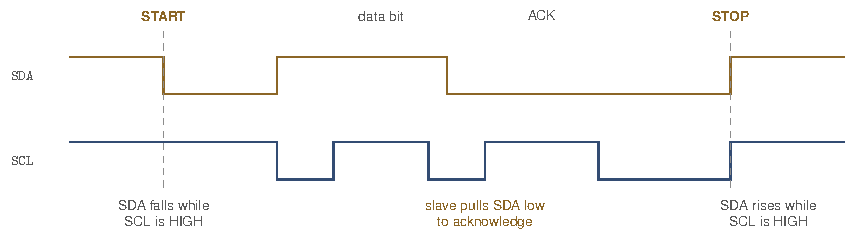
\includegraphics[width=.92\textwidth]{assets/i2c-framing.pdf}
    \end{center}

    \vspace{1mm}
    {\small\centering \texttt{SDA} may only change while \texttt{SCL} is LOW,
    so the two transitions that occur while \texttt{SCL} is HIGH are
    \alert{unambiguous markers} for the start and end of a transfer.\par}
\end{frame}

\begin{frame}{Addressing}
    \leavevmode
    Each device answers to a \alert{7-bit address}: 128 possibilities, a few reserved. The manufacturer fixes it, often with one or two pins to select between variants. That is how two identical sensors share one bus.

    \vspace{3mm}
    \begin{center}
    {\small
    \striped
    \begin{tabular}{@{}l l l@{}}
        \toprule
        \textbf{Datasheet says} & \textbf{On the wire, write} & \textbf{On the wire, read} \\
        \midrule
        \texttt{0x68} (7-bit) & \texttt{0xD0} & \texttt{0xD1} \\
        \bottomrule
    \end{tabular}}
    \end{center}

    \vspace{3mm}
    \begin{block}{A device that never acknowledges}
        The address goes in the upper seven bits of the first byte, with R/$\overline{\text{W}}$ in bit 0. A device that never ACKs is usually being addressed with the \alert{7-bit value shifted the wrong way}. The STM32 register expects the already-shifted 8-bit form.
    \end{block}
\end{frame}

\begin{frame}[plain]{Many Devices on Two Wires}
    \begin{center}
    \includegraphics[width=.86\textwidth, height=.6\textheight, keepaspectratio]%
        {assets/i2c-multi.pdf}
    \end{center}

    \vspace{1mm}
    {\small\centering Compare this with SPI's three private chip-select
    lines: here the pin count stays at \alert{two}, no matter how many
    devices hang off the bus --- selection has moved into \alert{software}.\par}
\end{frame}

\begin{frame}{I\textsuperscript{2}C Registers}
    \begin{center}
    {\scriptsize
    \striped
    \begin{tabular}{@{}l l l R{.46\textwidth}@{}}
        \toprule
        \textbf{Register} & \textbf{Bit} & \textbf{Name} & \textbf{Function} \\
        \midrule
        \texttt{I2C\_CR1} & 15 & \texttt{SWRST} & Software reset \\
                          & 10 & \texttt{ACK}   & Acknowledge enable; clear to NACK the next byte \\
                          & 9  & \texttt{STOP}  & Generate a stop condition \\
                          & 8  & \texttt{START} & Generate a start (or repeated start) \\
                          & 0  & \texttt{PE}    & Peripheral enable \\
        \texttt{I2C\_CR2} & 5:0 & \texttt{FREQ} & PCLK1 in MHz, used to time the bus \\
        \texttt{I2C\_CCR} & 11:0 & & $f_{\text{PCLK1}} / (2 \times f_{\text{SCL}})$ in standard mode \\
        \texttt{I2C\_TRISE} & 5:0 & & Maximum SCL rise time, in \texttt{FREQ} units \\
        \texttt{I2C\_SR1} & 7 & \texttt{TXE}  & Data register empty \\
                          & 6 & \texttt{RXNE} & A byte has arrived \\
                          & 2 & \texttt{BTF}  & Byte transfer finished \\
                          & 1 & \texttt{ADDR} & Address sent and acked; cleared by reading \texttt{SR1} then \texttt{SR2} \\
                          & 0 & \texttt{SB}   & Start condition generated \\
        \texttt{I2C\_SR2} & 1 & \texttt{BUSY} & Communication in progress \\
        \texttt{I2C\_DR}  & 7:0 &             & Carries the address byte and the data \\
        \bottomrule
    \end{tabular}}
    \end{center}

    \vspace{1mm}
    {\small The status bits are split across \alert{two} registers, \texttt{SR1} and \texttt{SR2}. This matters for \texttt{ADDR}.}
\end{frame}

\begin{frame}[fragile]{Configuring an I\textsuperscript{2}C Master}{I2C1 on PB8 (SCL) and PB9 (SDA), AF4}
    \begin{columns}[T]
    \begin{column}{.6\textwidth}
\begin{cc}[basicstyle=\ttfamily\scriptsize]
void i2c_init(void) {
    RCC->AHB1ENR |= (1U << 1);   // GPIOB
    RCC->APB1ENR |= (1U << 21);  // I2C1

    GPIOB->MODER &= ~((3U<<(8*2)) | (3U<<(9*2)));
    GPIOB->MODER |=  ((2U<<(8*2)) | (2U<<(9*2)));

    // OPEN-DRAIN. Without this the bus cannot work.
    GPIOB->OTYPER |= (1U << 8) | (1U << 9);

    // AF4 = I2C1; pins 8-15 are in AFR[1]
    GPIOB->AFR[1] &= ~((0xFU << 0) | (0xFU << 4));
    GPIOB->AFR[1] |=  ((4U << 0) | (4U << 4));

    I2C1->CR1 |= (1U << 15);     // SWRST
    I2C1->CR1 &= ~(1U << 15);    // release
    I2C1->CR2  = 16;             // FREQ: PCLK1 in MHz
    I2C1->CCR  = 80;             // 16 MHz / (2 x 100 kHz)
    I2C1->TRISE = 17;            // FREQ + 1
    I2C1->CR1 |= (1U << 0);      // PE
}
\end{cc}
    \end{column}
    \begin{column}{.36\textwidth}
        \begin{block}{The forgotten step}
            {\small Both pins must be \alert{open-drain} alternate-function outputs. This step has no counterpart in SPI, and it is the one most often forgotten.}
        \end{block}

        \vspace{2mm}
        \begin{center}
        \fbox{\parbox{.9\textwidth}{\centering\vspace{1mm}\small
        $\text{CCR} = \dfrac{f_{\text{PCLK1}}}{2 f_{\text{SCL}}} = 80$
        \vspace{1mm}}}
        \end{center}
        {\small \texttt{TRISE} $=$ \texttt{FREQ} $+ 1$ in standard mode.}
    \end{column}
    \end{columns}
\end{frame}

\begin{frame}[fragile]{A Register Read Over I\textsuperscript{2}C (1)}{Phases 1 and 2}
\begin{cc}[basicstyle=\ttfamily\footnotesize]
// addr: the 7-bit address ALREADY shifted left by 1
uint8_t i2c_read_reg(uint8_t addr, uint8_t reg) {
    while (I2C1->SR2 & (1U << 1)) { }     // bus free?

    // --- Phase 1: START, address for WRITE ---
    I2C1->CR1 |= (1U << 8);               // START
    while (!(I2C1->SR1 & (1U << 0))) { }  // SB: start sent
    I2C1->DR = addr & ~1U;                // address + write bit
    while (!(I2C1->SR1 & (1U << 1))) { }  // ADDR: address acked
    (void)I2C1->SR2;                      // SR1 then SR2 clears ADDR

    // --- Phase 2: send the register number ---
    while (!(I2C1->SR1 & (1U << 7))) { }  // TXE: DR empty
    I2C1->DR = reg;
    while (!(I2C1->SR1 & (1U << 2))) { }  // BTF: byte done
\end{cc}
    \vspace{1mm}
    {\small Each step waits on a status flag: the busy-wait pattern, applied to a peripheral whose every phase must be confirmed.}
\end{frame}

\begin{frame}[fragile]{A Register Read Over I\textsuperscript{2}C (2)}{Phases 3 and 4}
    \begin{columns}[T]
    \begin{column}{.62\textwidth}
\begin{cc}[basicstyle=\ttfamily\footnotesize]
    // --- Phase 3: repeated START, address for READ ---
    I2C1->CR1 |= (1U << 8);               // repeated START
    while (!(I2C1->SR1 & (1U << 0))) { }  // SB
    I2C1->DR = addr | 1U;                 // address + read bit
    while (!(I2C1->SR1 & (1U << 1))) { }  // ADDR
    I2C1->CR1 &= ~(1U << 10);             // ACK = 0: NACK
    (void)I2C1->SR2;                      // clear ADDR

    // --- Phase 4: receive one byte, then STOP ---
    I2C1->CR1 |= (1U << 9);               // STOP
    while (!(I2C1->SR1 & (1U << 6))) { }  // RXNE
    return (uint8_t)I2C1->DR;
}
\end{cc}
    \end{column}
    \begin{column}{.34\textwidth}
        \begin{block}{Two STM32 traps}
            {\small \texttt{ADDR} is cleared by reading \texttt{SR1} \emph{then} \texttt{SR2}. The \texttt{(void)I2C1->SR2} is not dead code: delete it and the bus hangs.

            \vspace{1mm}
            For a one-byte read, clear \texttt{ACK} \emph{before} clearing \texttt{ADDR}.}
        \end{block}
    \end{column}
    \end{columns}

    \vspace{1mm}
    {\small \textbf{Add a timeout} to every loop. A missing pull-up or an unpowered slave means a flag never sets, and the function never returns.}
\end{frame}

\begin{frame}{Choosing Between Them}
    \begin{center}
    {\small
    \striped
    \begin{tabular}{@{}l l l@{}}
        \toprule
         & \textbf{SPI} & \textbf{I\textsuperscript{2}C} \\
        \midrule
        Wires & 4, plus one CS \alert{per device} & \alert{2}, regardless of count \\
        Speed & \alert{Tens of MHz} & 100\,kHz to 1\,MHz \\
        Duplex & Full & Half \\
        Addressing & A chip-select line & A \alert{7-bit address} \\
        Acknowledge & None --- you cannot tell if it worked & \alert{ACK} per byte \\
        Best for & Displays, flash, fast ADCs & Many slow sensors, EEPROM \\
        \bottomrule
    \end{tabular}}
    \end{center}

    \vspace{3mm}
    \begin{block}{The trade in one sentence}
        \alert{SPI buys speed with pins}; \alert{I\textsuperscript{2}C buys pins
        with speed} --- and throws in an acknowledgement, so you know whether the
        device is actually there.
    \end{block}
\end{frame}


%===============================================================================
\section{Comparing the Serial Protocols}
%===============================================================================

\begin{frame}{Comparing the Serial Protocols}
    \begin{center}
    {\small
    \striped
    \begin{tabular}{@{}l l l l@{}}
        \toprule
        \textbf{Property} & \textbf{UART} & \textbf{SPI} & \textbf{I\textsuperscript{2}C} \\
        \midrule
        Clock & None (async) & Shared SCK & Shared SCL \\
        Wires & 2 & 4 (+1 per slave) & 2 \\
        Speed & to $\sim$1\,Mbps & tens of Mbps & 0.1--3.4\,Mbps \\
        Duplex & Full & Full & Half \\
        Devices & 2 & Many (one CS each) & Many (addressed) \\
        Addressing & None & Chip select & 7-bit address \\
        Typical use & PC terminal, GPS & Sensors, displays, SD & Small sensors, EEPROM \\
        \bottomrule
    \end{tabular}}
    \end{center}

    \vspace{3mm}
    \begin{block}{A NACK is diagnostic information}
        {\small I\textsuperscript{2}C is the only one with \alert{addressing in the protocol}, so it is the only one where a device can refuse to answer. An unpowered SPI slave returns \texttt{0x00} or \texttt{0xFF}, which looks like real data. An absent I\textsuperscript{2}C device announces its absence on the first byte.}
    \end{block}
\end{frame}


%===============================================================================
\section{Summary}
%===============================================================================

\begin{frame}{An SPI Byte at Five Levels}
    \begin{center}
    {\small
    \striped
    \begin{tabular}{@{}l R{.65\textwidth}@{}}
        \toprule
        \textbf{Level} & \textbf{Representation} \\
        \midrule
        Physical    & Eight clock pulses on PB13; data levels on PB15 and PB14 \\
        Hardware    & Two shift registers exchanging contents in a ring \\
        Register    & \texttt{SPI2->DR} written, then read \\
        C           & \texttt{value = spi\_transfer(0x00);} \\
        Engineering & One axis of acceleration, in units of g \\
        \bottomrule
    \end{tabular}}
    \end{center}

    \vspace{3mm}
    \begin{block}{You have now met every peripheral this book teaches}
        Digital pins, interrupts, timers, analog input, and three serial
        buses: one asynchronous and two synchronous. Chapter~14 asks you
        to use them \alert{all at once}, with no OS to arbitrate.
    \end{block}
\end{frame}

\begin{frame}{Summary}
	\begin{columns}[c]
		\begin{column}{.62\textwidth}
			\begin{center}
				\begin{tikzpicture}[x=10mm, y=7.8mm]
					\node[blk, minimum width=56mm, minimum height=5.0mm, inner sep=1.2pt, font=\scriptsize] (n0) at (0,0.00) {SPI: four wires, full duplex exchange};
					\node[blk, minimum width=56mm, minimum height=5.0mm, inner sep=1.2pt, font=\scriptsize] (n1) at (0,-1.05) {CPOL and CPHA give four modes};
					\node[blk, minimum width=56mm, minimum height=5.0mm, inner sep=1.2pt, font=\scriptsize] (n2) at (0,-2.10) {$f_{\text{SCK}} = f_{\text{PCLK}}/2^{(\text{BR}+1)}$; use SPI2};
					\node[blk, minimum width=56mm, minimum height=5.0mm, inner sep=1.2pt, font=\scriptsize] (n3) at (0,-3.15) {I\textsuperscript{2}C: two wires, addressed devices};
					\node[blk, minimum width=56mm, minimum height=5.0mm, inner sep=1.2pt, font=\scriptsize] (n4) at (0,-4.20) {Open-drain outputs, external pull-ups};
					\node[blk, minimum width=56mm, minimum height=5.0mm, inner sep=1.2pt, font=\scriptsize] (n5) at (0,-5.25) {START, address+RW, ACK, data, STOP};
					\node[blk, minimum width=56mm, minimum height=5.0mm, inner sep=1.2pt, font=\scriptsize] (n6) at (0,-6.30) {SPI: speed for pins. I\textsuperscript{2}C: pins for speed};
					\node[cpublk, minimum width=56mm, minimum height=5.0mm, inner sep=1.2pt, font=\scriptsize, align=center] (n7) at (0,-7.65) {Raw register values become\\engineering units};
					\foreach \a/\b in {0/1,1/2,2/3,3/4,4/5,5/6,6/7}{\draw[flow] (n\a) -- (n\b);}
				\end{tikzpicture}
			\end{center}
		\end{column}
		\begin{column}{.34\textwidth}
			{\scriptsize
				\textbf{Terminology covered}\\[1mm]
				\begin{itemize}
					\item MOSI, MISO, SCK, CS
					\item CPOL, CPHA
					\item Open-drain, pull-up
					\item START, ACK, STOP
				\end{itemize}
				\vspace{3mm}
				\textbf{Next: Chapter 14}\\[1mm]
				\emph{Designing, Building and Verifying}\\[1mm]
				Every peripheral so far, in one program, at once.}
		\end{column}
	\end{columns}
\end{frame}

\end{document}

